\chapter{Evaluation}
In this chapter, insights emanating from each queue's evaluation is compared
with findings from their seminal works; each queue's performance is compared, 
together with explanations as to why and what makes a queue superior to another.

\section{Workload under one thread}

\begin{figure}[!ht]
    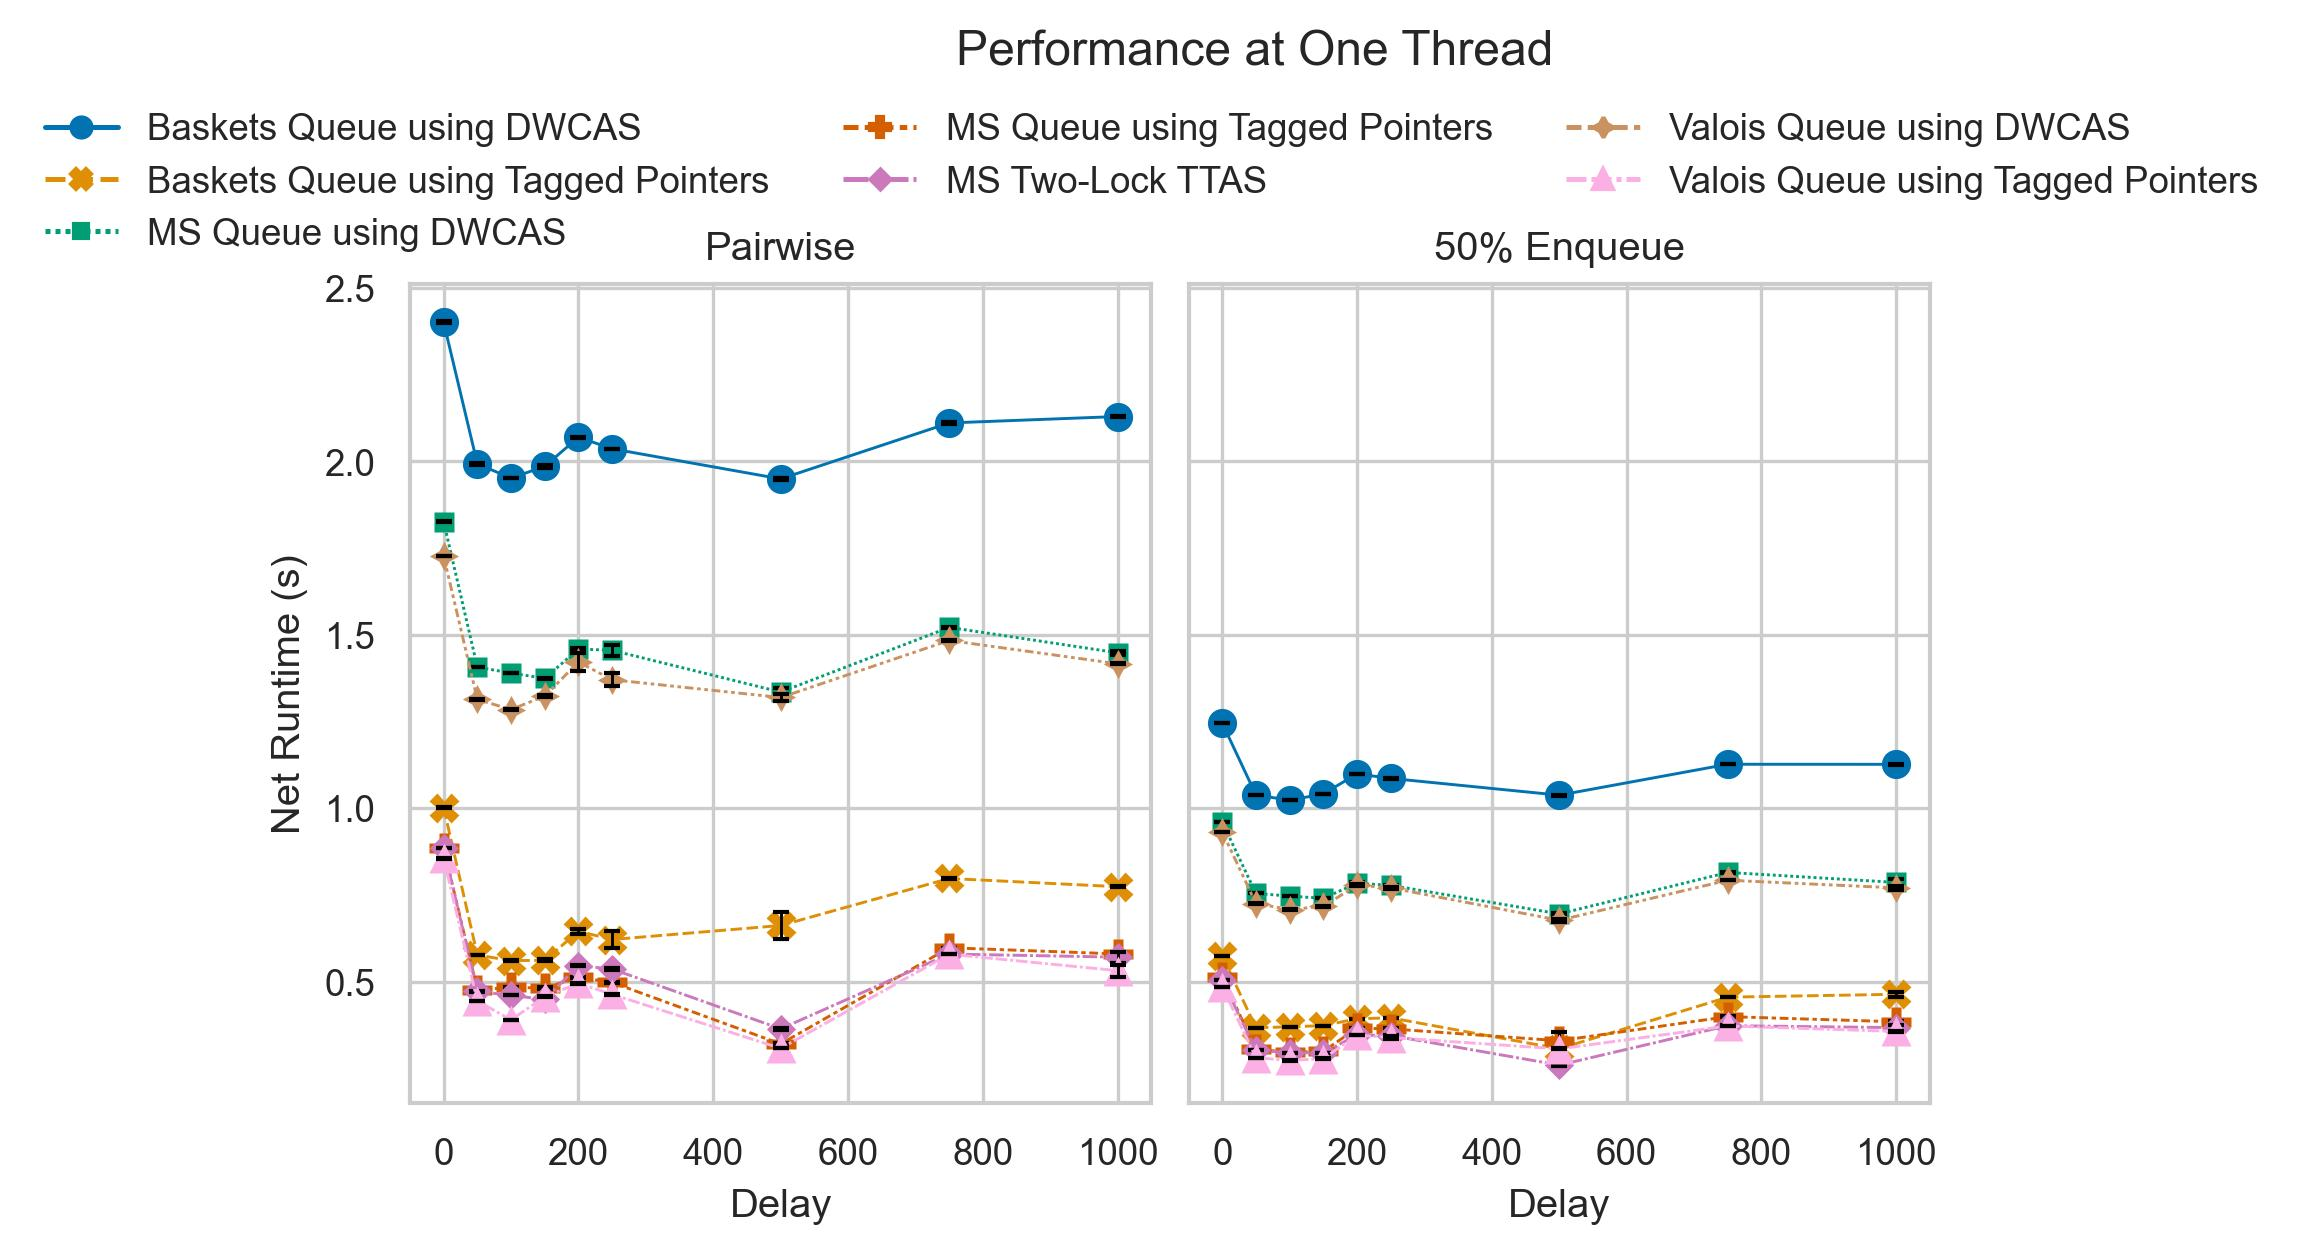
\includegraphics[width=1\textwidth,height=0.55\textwidth]{plots/delay_thread_1.jpg}
    \caption{The pairwise and the 50\% benchmarks on the left and right respectively.}
    \label{fig:perf_1_thread}
\end{figure}

The sequential latency of a queue is determined by its algorithmic
complexity~\citep{valois1995datastructures}. Contention-reducing mechanisms,
such as thread helping, are not triggered under single threaded workloads, as
they rely on failed Compare-and-Swaps, adding extra overhead through the
computation of predicates. Figure \ref{fig:perf_1_thread} shows the performance
of each queue in a single threaded workload; Nonblocking queues using
tagged pointers perform twice as fast as their DWCAS counterparts.  
Most queues achieve optimal performance at a delay of 500 nanoseconds, with
the exception being the baskets queue using tagged pointers, due to its more
elaborate contention-reducing mechanisms.

\section{Workload under two threads}
Similar to \citep{michael1996simple,hoffman2007baskets,ladan2008optimistic},
under a workload of two threads, a significant degradation in performance can
be observed. \citeauthor{michael1996simple} notes that as each queue's head and
tail are shared across two processors, cache misses are more frequent. Figure
\ref{fig:perf_deg_1_thread} shows the ratio of time taken between two-threaded
and single threaded workloads, which represent the magnitude of performance
degradation between both workloads. Queues using tagged pointers tend to
experience higher contention, consequently leading to a harsher degradation in
performance; in support of this claim, the Baskets Queue using Tagged pointers
with zero delay was \textbf{61\%} more likely to re-attempt an enqueue\footnote{This metric was gathered by
incrementing an integer (found in thread local storage) every time it repeated
anything past line \emph{E03} of the Baskets Queue.} than its DWCAS counterpart.

\begin{figure}[!ht]
    \centering
    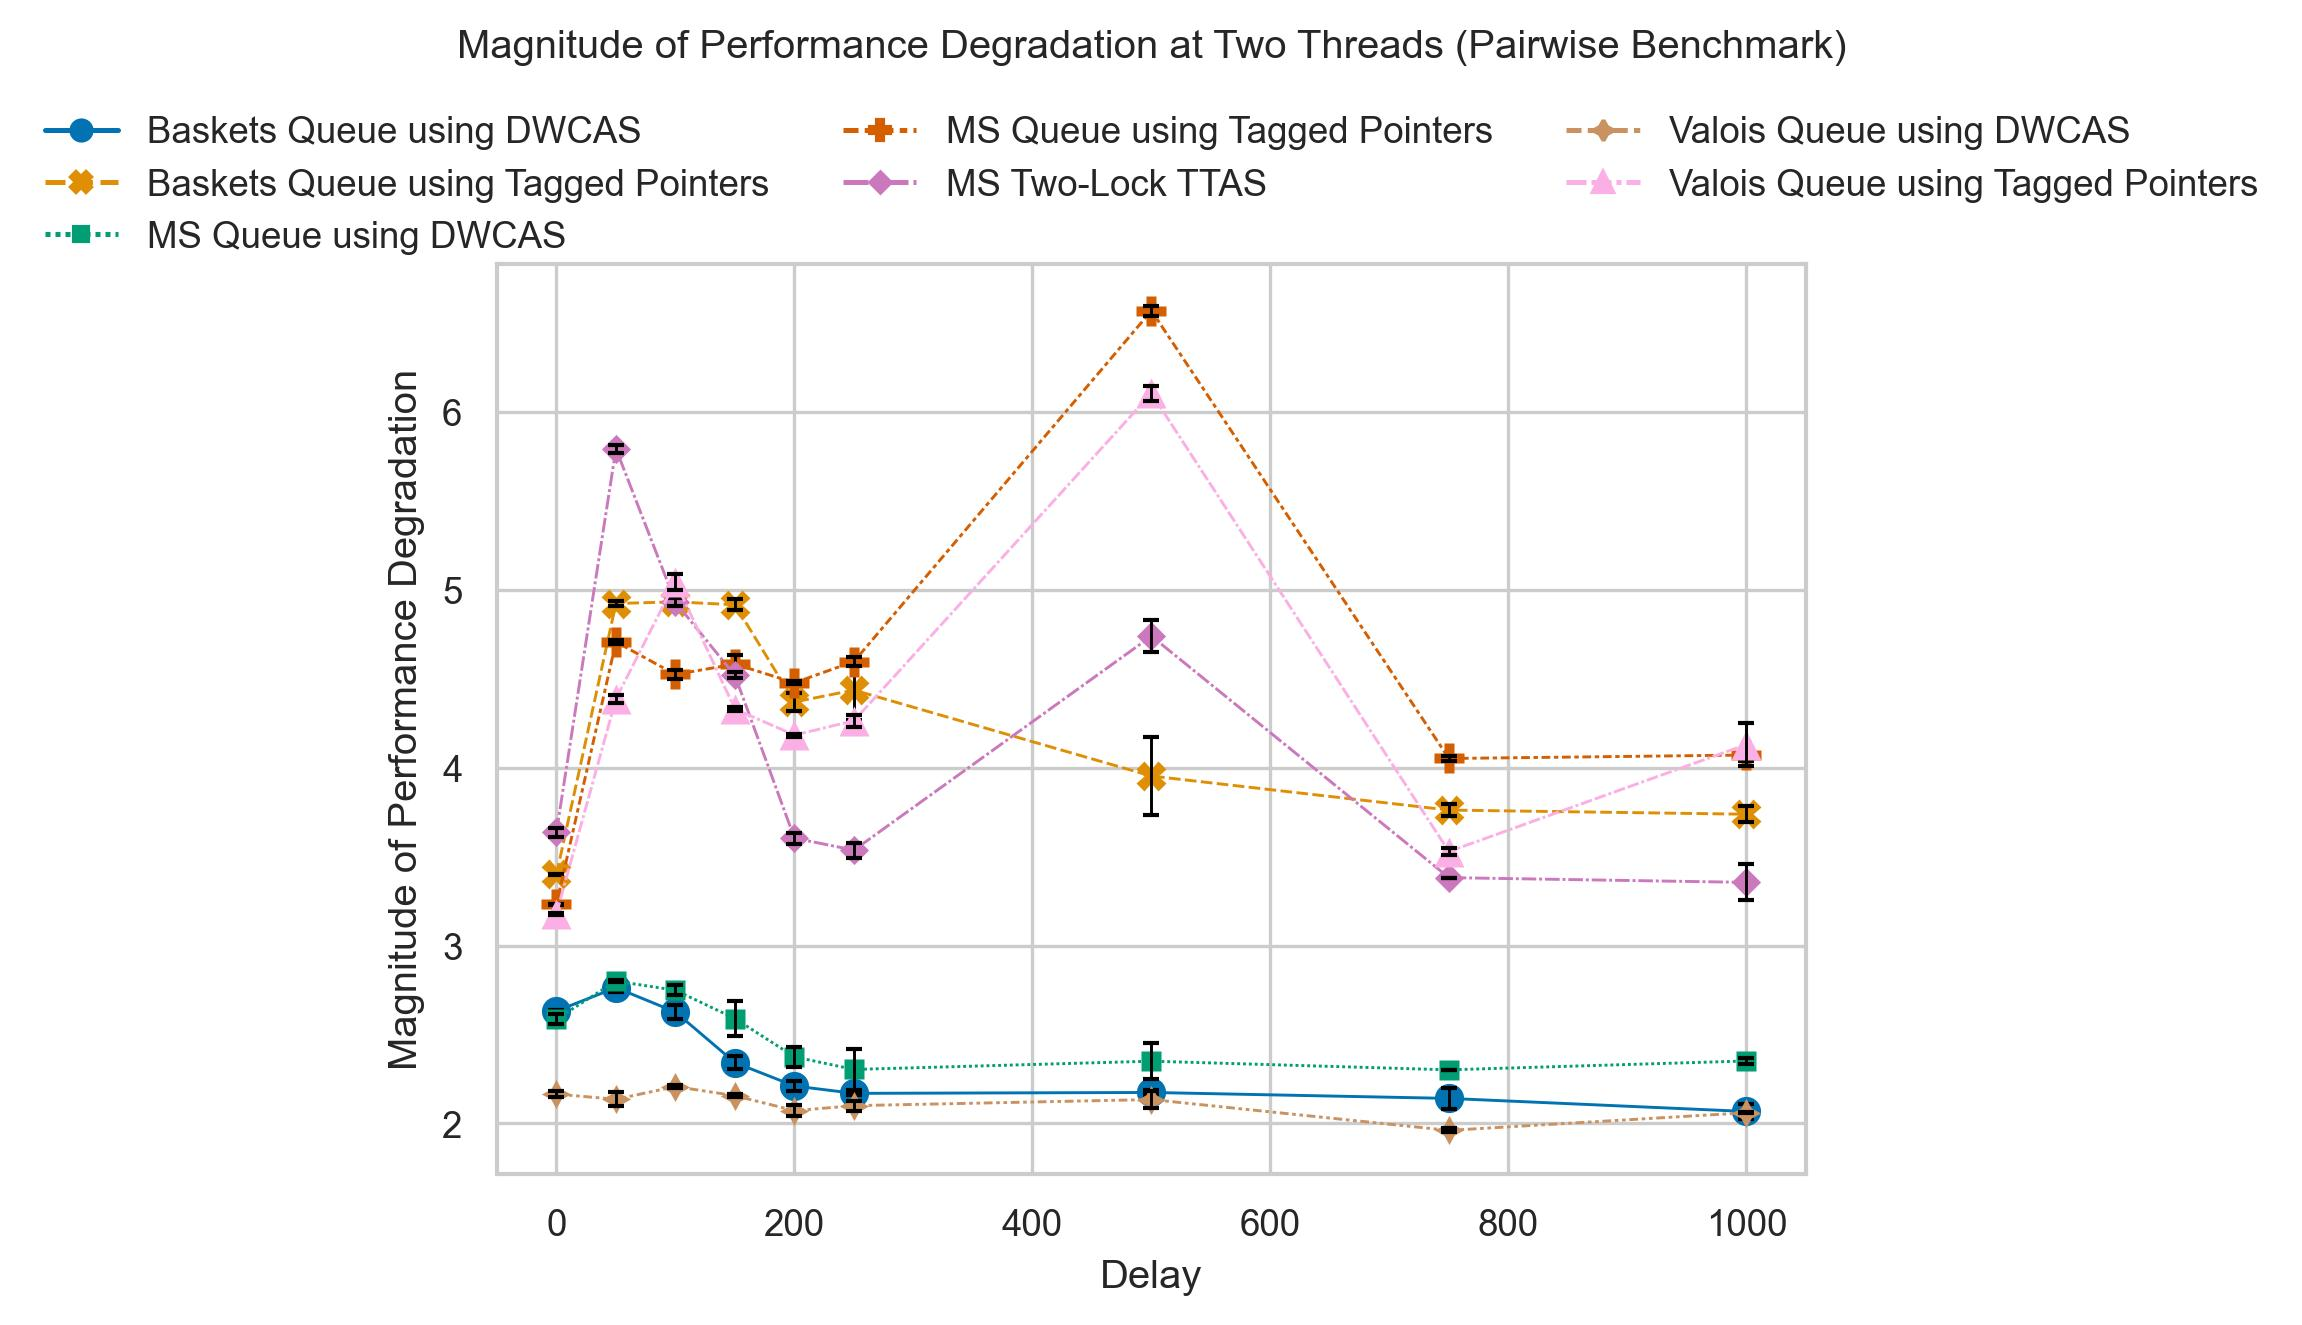
\includegraphics[width=1\textwidth]{plots/speedup_enqueue_dequeue_1.jpg}
    \caption{The magnitude of performance degradation between single and two-threaded workloads.}
    \label{fig:perf_deg_1_thread}
\end{figure}

\begin{figure}[!ht]
    \centering
    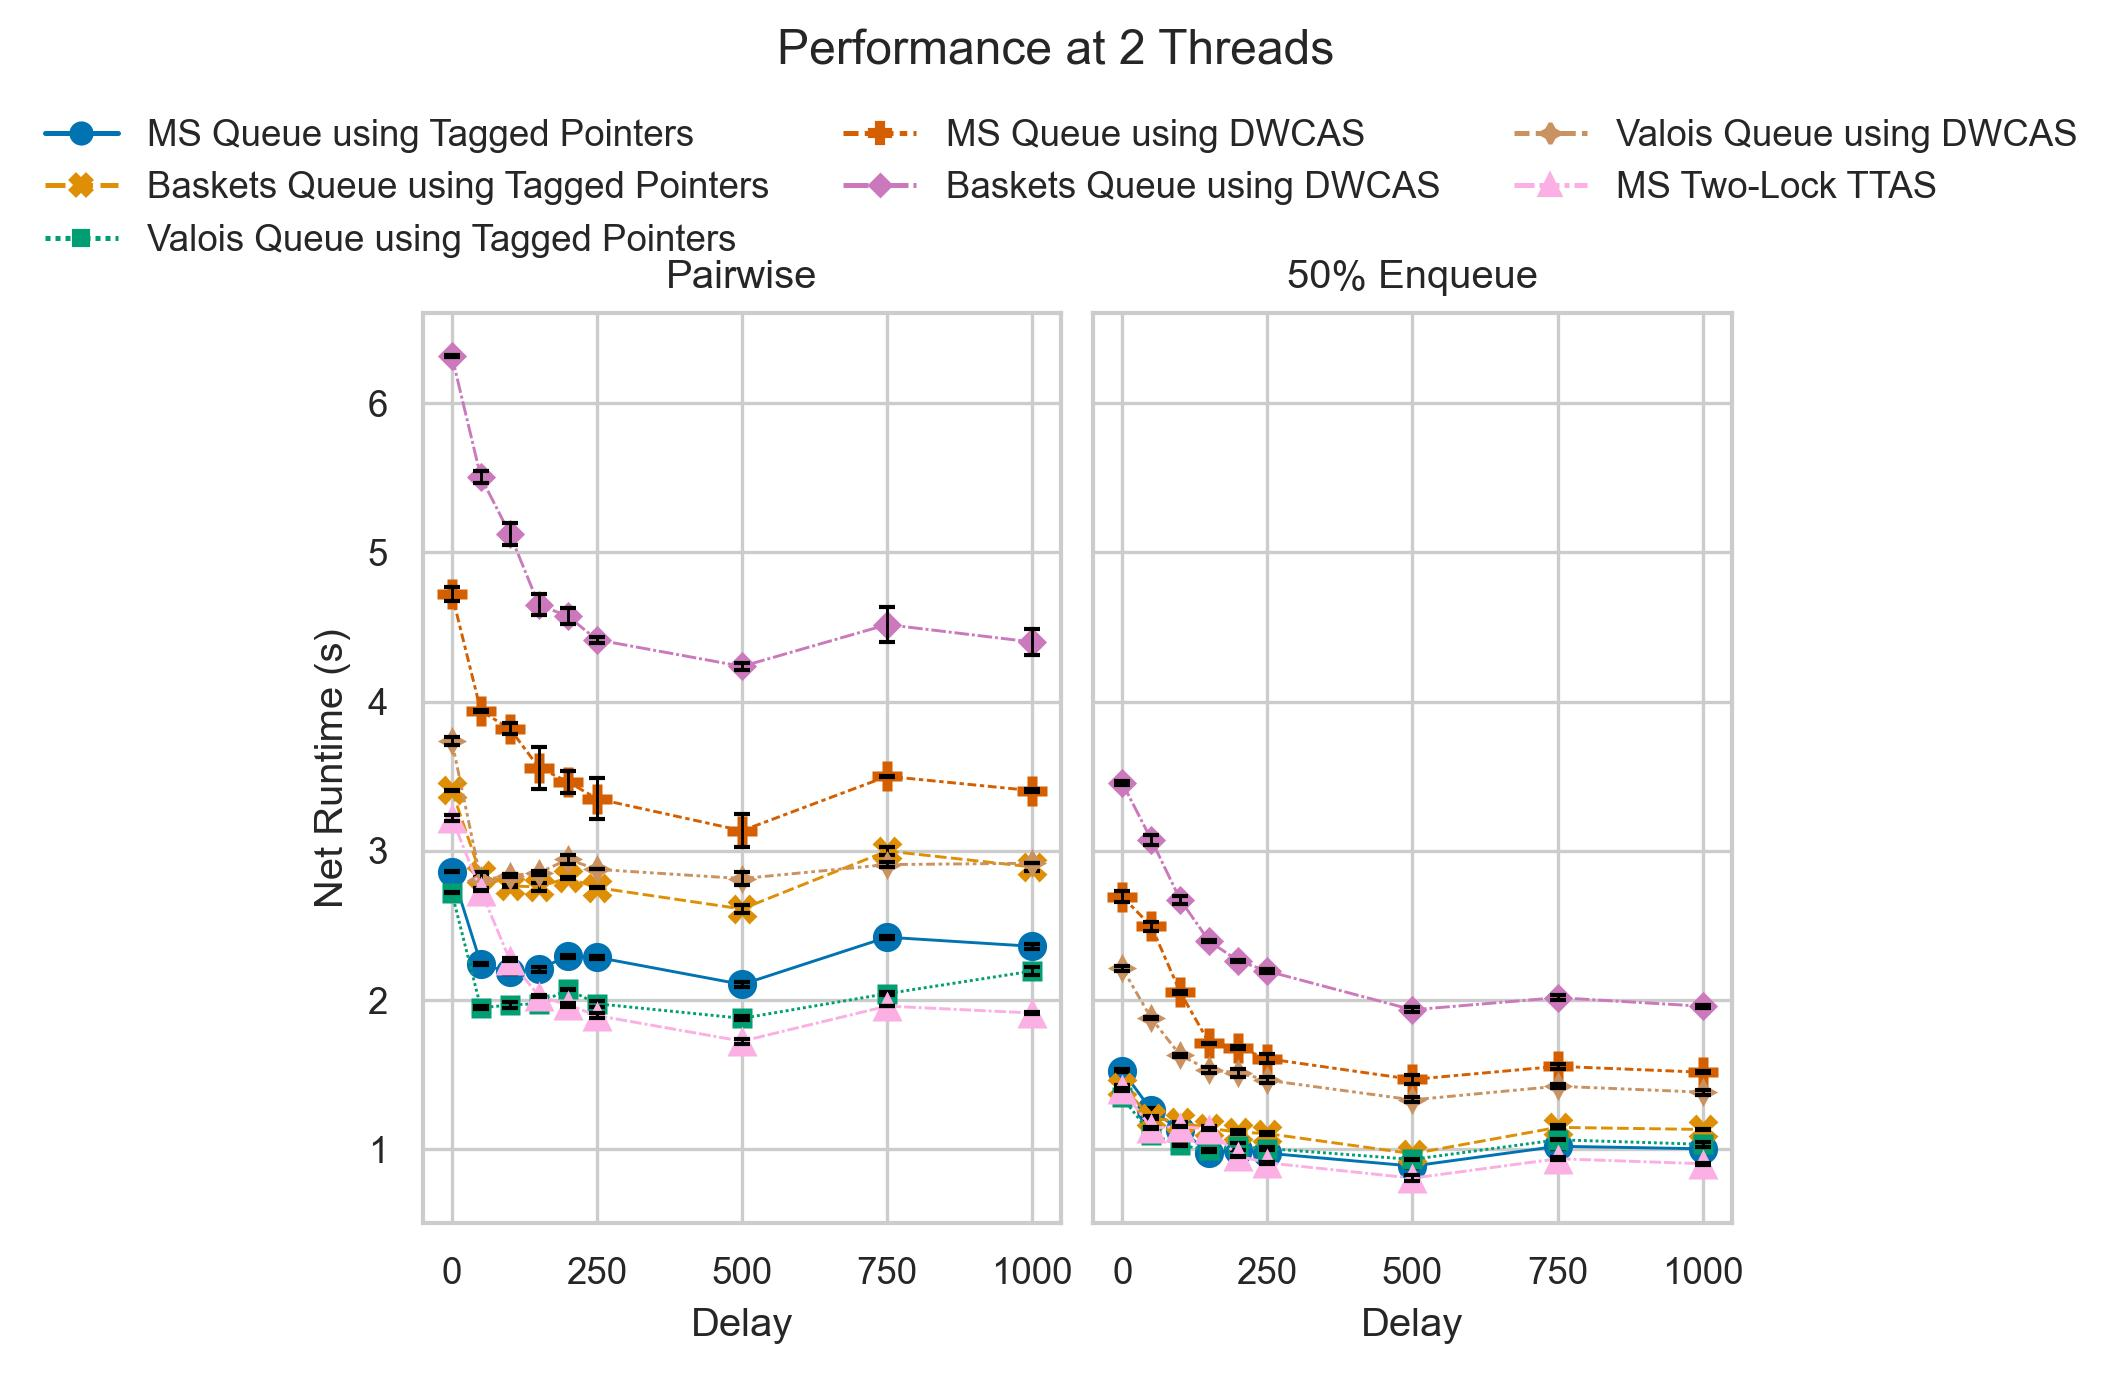
\includegraphics[width=1\textwidth]{plots/delay_thread_2.jpg}
    \caption{The pairwise and the 50\% benchmarks on the left and right respectively.}
    \label{fig:perf_2_thread}
\end{figure}

At delays greater than 200 nanoseconds, the two-lock queue exhibits the best
performance; nonblocking queues using tagged pointers remain competitive in
low-contention scenarios. 

The performance of \citeauthor{valois1994queues}' queue in this study highly
conflicts with that of \citep{michael1996simple}. Although a queue without a
memory reclamation scheme may share a common algorithm with one that has, it
does not imply that they are algorithmically equivalent, making their
performance unconnected; as this study does not include memory reclamation
schemes in its implementations, valid comparisons cannot be made with
~\citep{michael1996simple}'s results of \citeauthor{valois1994queues}' queue,
however, insights may still be inferred.
\citeauthor{michael1996simple}\textemdash conveniently\textemdash fail to
disclose that memory reclamation overheads were excluded from the reported
performance of the MS-queue, leading to biased comparisons against other
queues.

One may hypothesize \citeauthor{valois1994queues}' queue fitted with the \emph{safe read}
protocol leads to a horribly inefficient algorithm, as each enqueueing thread
is required to traverse part of the linked list, incurring a high number of
cache misses, since a reference counter has to be modified twice with each
traversal (once to reclaim a node, and another to release it).

\section{Workload Under Three Threads}
In \citep{ladan2008optimistic,michael1996simple,hoffman2007baskets},
a minor improvement in performance under three threads is observed;
\citeauthor{michael1996simple} link the boost in performance to the fewer
iterations per thread, combined with a cache miss rate similar to that under
two threads.

% \section{Biases and Threats to Validity}
% \paragraph{Artificiality of Workloads}
% In \citep{gregg2014systems}, \citeauthor{gregg2014systems} claims that
% \emph{micro-benchmarks} (type of benchmark adopted in this study) produces
% artificial workloads, rendering results which are  solely obtained under
% various assumptions. Results obtained in this study represent the concurrent
% queues, whose operations are separated by fixed delays, inside a ``clean-room''
% environment. Realistic workloads seldom follow such rigid patterns, making the
% results' validity under real-world scenarios undetermined.

% \paragraph{Impact of Consumer Grade CPUs on Performance}
% For the scope of this study, cutting-edge hardware, similar to that used in
% prior art, is inaccessible. Unfortunately, over-subscription of processors
% is required to gather enough an acceptable amount of data, making it
% impossible to reproduce trends solely attainable from low-degrees of over-subscription. At
% best, the resources accessible to the study may only produce
% highly-multiprocessed workloads.
